\documentclass[font=default]{mpltx}
\usepackage{bm, ctex}
\usepackage{subfigure}
\usepackage{multirow}
% 以下至 \begin{document} 都仅是本文件为了方便额外定义的命令, 写报告时不需要.
\hypersetup{colorlinks=false}% 超链接带颜色
\usepackage{xcolor}
% 以上是本文件为了方便额外定义的命令, 写报告时不需要.
\linespread{1.5}
\begin{document}

\title{硅的系数及电阻率的测量} % 切合报告内容, 简短明确, 可以不同于讲义
\author{MaskedName} % 这里 \emailphone 一定要紧跟在 \author 后方
\emailphone{MyMail@stu.pku.edu.cn}{Tel}
% 如果改用 \email 则仅需要邮箱参数
\affiliation{北京大学物理学院\quad 学号: StudentID}
\date{\zhdate{2023/11/1}}
\begin{abstract}
当测定导体的电阻率和霍尔系数时,我们可以获取有关其基本电学特性的信息,这有助于我们理解和验证导电机理。本实验旨在将这种方法应用于半导体的研究,旨在通过测定p型硅的电阻率和霍尔系数,来验证半导体的导电特性和机理。在本实验中,我们采用范德堡法来测量了从室温至150°C范围内p型硅的电阻率和霍尔系数。我们获得并分析了霍尔系数和电阻率随温度的变化关系,从而验证了固体理论对掺杂半导体的导电机制的预测。此外,我们还成功确定了所用样品p型硅的禁带宽度$E_g$。
\end{abstract}
\keywords{半导体理论,能带理论,霍尔效应,范德堡法}

\maketitle

\section{引言}
半导体科学的进步和发展是推动社会进步的最重要的推力之一。半导体技术的研究和突破,总会在各个领域引起新的革命和快速发展。早在19世纪,人们就认识到了半导体不同寻常的性质,并展开了对半导体的研究,并在后来的发展中,人们不断地揭示了电子在半导体内部各种形式的运动,并逐步阐明了它的规律性。

1878 年,霍尔(Edwin Herbert Hall)指出,磁场会导致导体中的载流子发生偏
转,电荷在导体侧面累积产生可测的电压,电压正负取决于载流子类型;此即霍尔效
应。随后的 1897 年,J. J. 汤姆孙(Sir Joseph John Thomson)发现电子,结合霍尔效应的结论,人们猜想,导体中的电流由电子定向漂移形成。此后,人们发现了两种霍尔效应,例如,与导体不同,CuI应当具有正电荷载流子,但人们当时并不清楚这一正电荷载流子究竟由何种粒子构成。

20世纪上半叶发展出来的量子力学和固体理论解释了这个问题。1931 年,由威尔逊(Alan Herries Wilson)等人提出的能带理论得以确立,统一地解释了导体和半导体的导电特性,并且揭示了半导体在不同温度下电阻和霍尔系数的变化规律。

本实验测量了p型半导体样品在室温(\textasciitilde$25^\circ$C)到150$^\circ$C左右的电阻率和霍尔系数。并通过实验结果测量载流子的浓度和迁移率,检验了固体理
论给出的预测,从而对理论有了更加深刻的理解。此外,本实验还计算了禁带宽度等其他关于材料的基本参数。
\section{理论}
\subsection{电导率和温度的关系}
% $$\mbox{\CJKfamily{zhkai}没问题}$$
固体理论中,半导体的导电机制有两种:一是半导体自身晶格电子由热激发(本征激发)从价带进入导带,产生载流子导电,称为本征导电;二是由杂质引入的额外电子、空穴所带来的导电效应,称为杂质导电。

一般的半导体中,这两种导电效应都存在,并且随着温度变化,不同机制产生的效应变化不同,因此半导体的导电性质会随着温度变化。定义迁移率$\mu$为
\begin{equation}\bm{v}_d=\mu\bm{E}.\end{equation}
其中$\bm{v}_d$为载流子的漂流速度。对于p型硅,我们记
$$\begin{array}{rl}
  N_A &\mbox{\CJKfamily{zhkai}为杂质浓度},\\
  p_s &\mbox{\CJKfamily{zhkai}为杂质电离产生的空穴浓度},\\
  p &\mbox{\CJKfamily{zhkai}为空穴总浓度},\\
  n &\mbox{\CJKfamily{zhkai}为电子总浓度}.
\end{array}$$于是电导可表示为迁移率和载流子浓度的乘积
\begin{equation}\label{sigma}
  \sigma=nq\mu_{\rm n}+pq\mu_{\rm p}=q\mu_{\rm p}(bn+p).
\end{equation}其中$\mu_{\rm n}$和$\mu_{\rm p}$电子和空穴的晶格散射迁移率,$b=\mu_{\rm n}/\mu_{\rm p}$。

电导率$\sigma$随温度$T$的变化如图\ref{ln_sigma_1_T}所示,这里可以分为三个区域\cite{book}。

1.\textbf{杂质部分电离的低温区}。在这个区域载流子主要是杂质电离的空穴或电子,随着温度升高,载流子不断被电离。迁移率$\mu_{\rm p}$主要取决于杂质散射,随温度缓慢增加,因此电导率随着温度的升高而增加。

2.\textbf{杂质电离饱和的温度区}。在这个区域载杂质已被全部电离,但是本征激发还不明显,所以载流子浓度基本不变。这时晶格散射起主要作用,随着温度升高晶格散射越来越强,迁移率$\mu_{\rm p}$不断下降,因此电导率随着温度的升高而降低。\\在300 K温度下,p型硅的电导率取决于晶格散射的空穴迁移率$(\mu_{\rm L_p})_{300}=480\ {\rm cm^2/(V\cdot s)}$。在杂质电离饱和区内其他温度的迁移率$(\mu_{\rm L_p})_T$和$(\mu_{\rm L_p})_{300}$有如下关系\begin{equation}\label{mu_LP}
  (\mu_{\rm L_p})_T=(\mu_{\rm L_p})_{300}\frac{\sigma_T}{\sigma_{300}}.
\end{equation}可通过这个关系式求$(\mu_{\rm L_p})_T$随温度的变化曲线。

3.\textbf{产生本征激发的高温区}。在这个区域中,本征激发显著,半导体成对地产生电子和空穴,且$n$、$p$随指数增大,由电荷守恒我们有$p = p_s + n = N_A + n$。迁移率依然为下降趋势,但仅仅是按幂律减小,因此电导率随温度的上升急剧增大。根据摩润(Morin)等人的研究结果,在本征激发的高温区,$\mu_{\rm L_p}$和$\mu_{\rm L_n}$和温度有如下关系\cite{Morin}\begin{equation}\label{Morinresult}
  \begin{aligned}
    \mu_{\rm L_n}=4.0\times10^9T^{-2.6}\ {\rm cm^2/(V\cdot s)},\\
    \mu_{\rm L_p}=2.5\times10^8T^{-2.3}\ {\rm cm^2/(V\cdot s)}.
  \end{aligned}
\end{equation}

将电荷守恒一式代入式\ref{sigma}可得到\begin{equation}\label{p_expression}
  \begin{aligned}p&=\frac{\frac{\sigma}{q\mu_{\rm L_p}}+bp_s}{b+1},\\n&=\frac{\frac{\sigma}{q\mu_{\rm L_p}}-p_s}{b+1}.\end{aligned}
\end{equation}利用关系式$np\propto AT^3\exp(-E_g/kT)$,作出$\ln(npT^{-3})-(1/T)$曲线,用最小二乘法可以确定禁带宽度\begin{equation}\label{DeltaEg}
  E_g=\frac{k\Delta\ln(npT^{-3})}{\Delta\left(\dfrac1T\right)}.
\end{equation}
\begin{figure}[h]
  \centering
  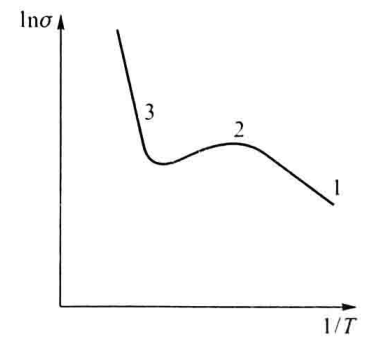
\includegraphics[width=0.3\linewidth]{fig/ln_sigma_1_T.png}
  \caption{硅的$\ln\sigma-(1/T)$曲线}
  \label{ln_sigma_1_T}
\end{figure}

\subsection{霍尔效应}
磁场与电流方向正交时,洛伦兹力导致载流子沿与电流和磁场垂直的方向运动,这样就会在导体的侧面积累电荷,从而产生电势差。由电磁学知识,我们很容易得到p型半导体的霍尔系数$R_H$为\begin{equation}
  R_H=\frac{1}{pq},\quad V_H=R_H\frac{IB}{d}\ \mbox{\CJKfamily{zhkai}为霍尔电压}.
\end{equation}但是上述结论是在所有载流子都以相同速度运动的假设下获得的,事实上,载流子的运动在复杂得多。更细致的分析表明,在球形等能面下,只考虑晶格散射和弱磁场近似,霍尔系数为\cite{book}\begin{equation}\label{Hall_coefficient}
  R_H=\frac{3\pi(p-nb^2)}{8q(n+nb)^2},\quad b=\frac{\mu_{\rm n}}{\mu_{\rm p}}.
\end{equation}这里$b>1$,即电子的迁移率高于空穴。

我们可以简要分析p型半导体中$R_H$随温度增大的变化规律。

1.较低温时,杂质电离饱和(对应图\ref{ln_sigma_1_T}电导变化的第2阶段)。此时p型半导体中$p\gg n$,载流子几乎为空穴且浓度基本不变,霍尔系数$R_H$近似为常数,这也是我们在电磁学中得到的结论。

2.温度逐渐升高时,本征激发开始(对应图\ref{ln_sigma_1_T}电导变化的第3阶段前半部分)。此时电子浓度$n$显著增大,导致霍尔系数$R_H$随温度升高不断减小,当温度升高到$p=nb^2$时,有$R_H=0$。

3.温度再升高时,更多的电子被激发到导带(对应图\ref{ln_sigma_1_T}电导变化的第3阶段后半部分)。这时$p<nb^2$因此$R_H<0$,最终空穴和电子数量相当,根据式\ref{Hall_coefficient}最终$R_H\to 0$,所以霍尔系数一定会出现极值。事实上,将$p=n+N_A$代入式\ref{Hall_coefficient}并求导数,可以得到,当$n=N_A/(b-1)$时,$R_H$达到极值\begin{equation}\label{R_Hmin}
  (R_H)_{\min}=-R_{\rm H,s}\frac{(b-1)^2}{4b},\quad R_{\rm H,s}=\frac{3\pi}{8}\frac{1}{N_Aq}.
\end{equation}这里的$R_{\rm H,s}$是杂质电离饱和区的霍尔系数,据此我们可以估算$b$。

\subsection{范德堡法测量任意形状薄片的电阻率及霍尔系数}
对于如图\ref{arb_sample}所示的任意形状的样品(中间没有空洞),其厚度为$d$,可以证明电阻率和霍尔系数为\cite{Pauw}\begin{equation}
  \rho=\frac{\pi d}{\ln 2}\frac{R_{12,34}+R_{23,41}}{2}f,\quad R_H=\frac{d}{B}\Delta R_{12,34}.
\end{equation}
式中$$R_{\alpha\beta,\gamma\delta}=\frac{V_\delta-V_\gamma}{i_{\alpha\beta}},$$其中$i_{\alpha\beta}$表示从$\alpha$端流向$\beta$端的电流,$V_\gamma$表示$\gamma$端的电位$(\{\alpha,\beta,\gamma,\delta\}=\{1,2,3,4\})$。$f$是对称性因子,对于本实验采用的样品$f\approx 1$。求霍尔系数时,$\Delta$表示加磁场前后测量到的电阻差。这一测量方法首先由范德堡(Van der Pauw)提出,本实验即采用这一办法测定电阻率$\rho$和霍尔系数$R_H$。

\begin{figure}[h]
  \centering
  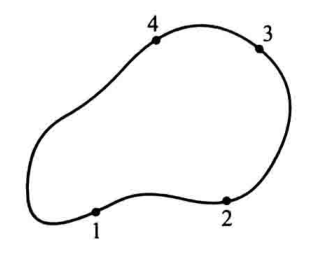
\includegraphics[width=0.3\linewidth]{fig/arb_sample.png}
  \caption{任意形状的样品}
  \label{arb_sample}
\end{figure}
\section{实验内容}
\subsection{实验装置}
本实验中的磁场由永磁魔环提供,磁场强度恒定$B\approx0.38$ T,在实验过程中我们只改变磁场方向而不改变磁场大小。我们采用恒流电源$I=(100.00\pm0.02)\ {\rm \mu A}$,所使用的样品厚度为$d=(1.00\pm0.02)\ {\rm mm}$。

实验主要通过BWH-1型霍尔效应测试仪进行样品加热以及供电、测温、测压等。实验采用铜-康铜温差电偶测量样品温度(实验操作手册附录给出铜-康铜温差电偶电势为$\epsilon=at+bt^2+ct^3$(单位:mV),其中$a=3.827\times10^{-2},b=5.59\times10^{-5},c=-1.06\times10^{-7}$,$t$的单位为$^\circ{\rm C}$\cite{manual})。

\subsection{实验过程}
\subsubsection{测量室温条件下的电阻率和霍尔系数}
开启BMH-1型霍尔效应测试仪的总电源开关,调节电流输出使测量电流为$100.00{\rm \mu A}$。依次测量$V_{\uppercase\expandafter{\romannumeral1}}$和$-V_{\uppercase\expandafter{\romannumeral1}}$、$V_{\uppercase\expandafter{\romannumeral2}}$和$-V_{\uppercase\expandafter{\romannumeral2}}$、$V_{\uppercase\expandafter{\romannumeral3}}(0,+I)$和$-V_{\uppercase\expandafter{\romannumeral3}}(+B,+I)$、$V_{\uppercase\expandafter{\romannumeral3}}(0,-I)$和$-V_{\uppercase\expandafter{\romannumeral3}}(-B,-I)$。通过电流、磁场换向测量并且取平均值,可以消除大部分热副效应\cite{book}。

\subsubsection{测量室温到$165\ ^\circ{\rm C}$温度范围内样品的电阻率和霍尔系数}
“温度控制仪”的设定值选择40,50,60,70,80,90,100,107,114,121,128,135,141,144,147,150,153,156,159,162,166$^\circ{\rm C}$。待温度稳定后(实际上由于各种热效应,样品的温度会低于设置的温度,所以需要同时记录样品的温度),重复上面的测量,并列表。

注意在测量过程中,温度在达到平衡附近会有略微的振荡。待温度波动最小后,记录样品温度,并且快速改变电流和磁场依次测量上述数据。一组读数完成后,若样品温度变化不大,则认为数据有效,否则应该等待温度达到平衡状态后重新进行测量。

\section{实验结果与分析}
\subsection{不同温度下的电阻率和霍尔系数}
测量不同温度下的电阻率和霍尔系数的结果如图\ref{T_rho_RH}所示。作$\ln\rho-(1000/T)$和$\ln |R_H|-(1000/T)$曲线如图所示。

将图\ref{Tln_rho_RH}和图\ref{ln_sigma_1_T}进行对比(因为$\rho=1/\sigma$,所以单调性的分析应该相反),可以得到实验中所取的温度实际上对应着半导体的(2)杂质电离饱和区和(3)本征激发区。

从室温(约为25$^\circ$C)到约50$^\circ$C范围内,电阻率$\rho$随着温度的升高而增大,这说明此时杂质电离已经饱和,晶格散射起主要作用,对应的是杂志电离饱和的温度区。在50$^\circ$C,$\rho$迅速减小,说明材料进入了本征激发的高温区,半导体内的载流子数目快速增加。

随后我们计算半导体中杂质的浓度$N_A$。在300 K温度下,p型硅的空穴迁移率为$(\mu_{\rm L_p})_{300}=480\ {\rm cm^2/(V\cdot s)}$。我们可以通过图\ref{T_rho_RH}中的数据进行内插得到300 K下的电阻率是$(\rho)_{300}=3182\ \Omega\cdot{\rm cm}$。从而根据$1/\rho=\sigma\approx qN_A\mu_{\rm L_p}$,我们可以得到杂质的浓度\begin{equation}\label{NA_value}
  N_A=4.1\times10^{12}\ cm^{-3}.
\end{equation}

得到了半导体中杂质的浓度,我们就可以计算实验中最高测量温度下的空穴浓度。最高测量温度下的测定值$$T_{\max}=156.4^\circ{\rm C},\quad \rho=251.8\ \Omega\cdot{\rm cm},\quad R_H=-8.55\times10^4\ {\rm cm^3\cdot C},$$将数据代入式\ref{p_expression},其中迁移率$\mu_{\rm L_p}$可以使用Morin等人的研究结果(见式\ref{Morinresult})进行计算。最终我们得到最高温度下,半导体样品的空穴浓度为\begin{equation}\label{p_max_value}p=3.6\times10^{13}\ {\rm cm^{-3}}.\end{equation}
比较式\ref{NA_value}和式\ref{p_max_value},可以知道在实验中的最高测量温度下,空穴浓度比杂质浓度大出一个数量级,表明此时本征激发电离出的电子空穴对已经充分的多,也就是样品已经完全进入本征激发的范围。
\begin{figure}[h]
  \centering
  \setlength{\abovecaptionskip}{-0.4cm}
  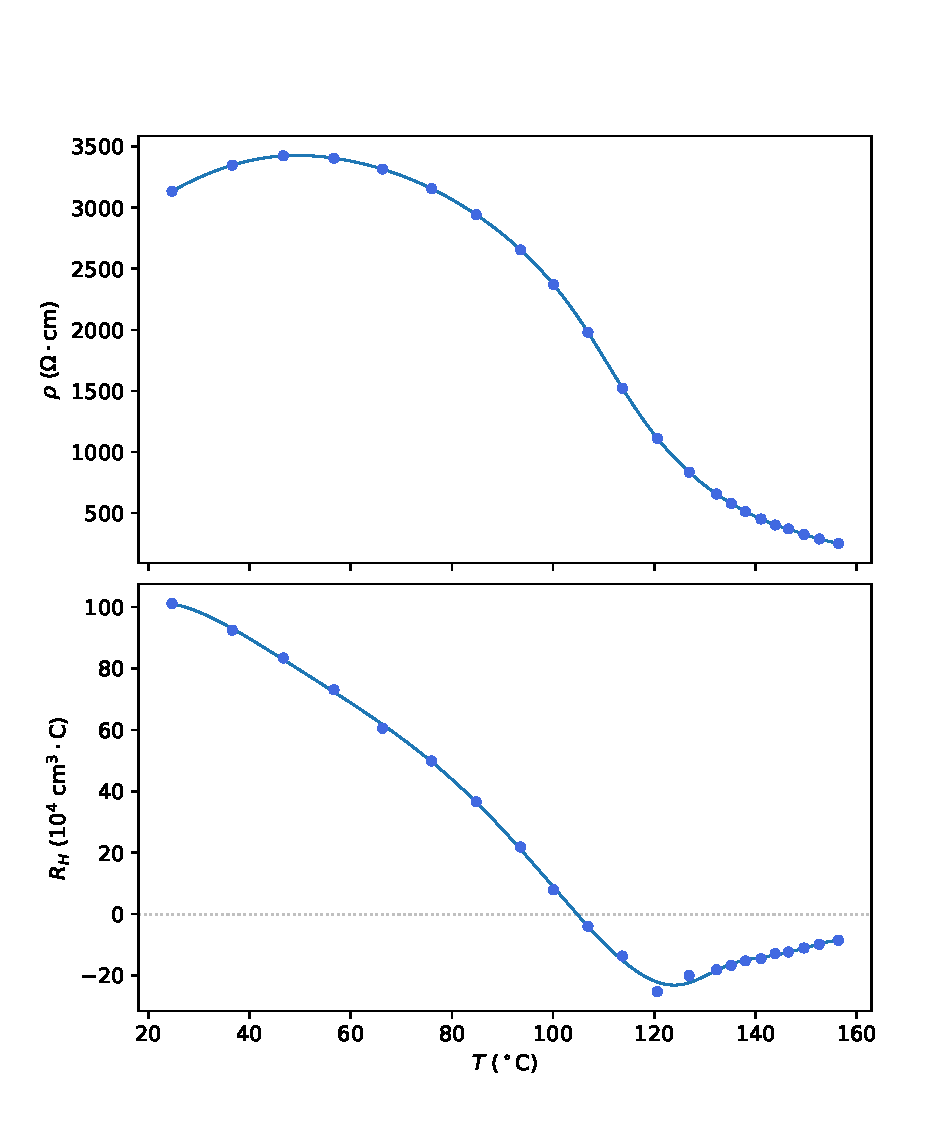
\includegraphics[width=0.8\linewidth]{fig/T_rho_RH.pdf}
  \caption{实验测量电阻率$\rho\ (\Omega{\rm \cdot cm})$和霍尔系数$R_H\ ({\rm cm^3\cdot C})$随温度$T\ ({\rm ^\circ C})$变化的图像。曲线由三次样条拟合给出。霍尔系数约在$T=104.5\ {\rm ^\circ C}$处变为零。}
  \label{T_rho_RH}
\end{figure}

\begin{figure}[h]
  \centering
  \setlength{\abovecaptionskip}{-0.4cm}
  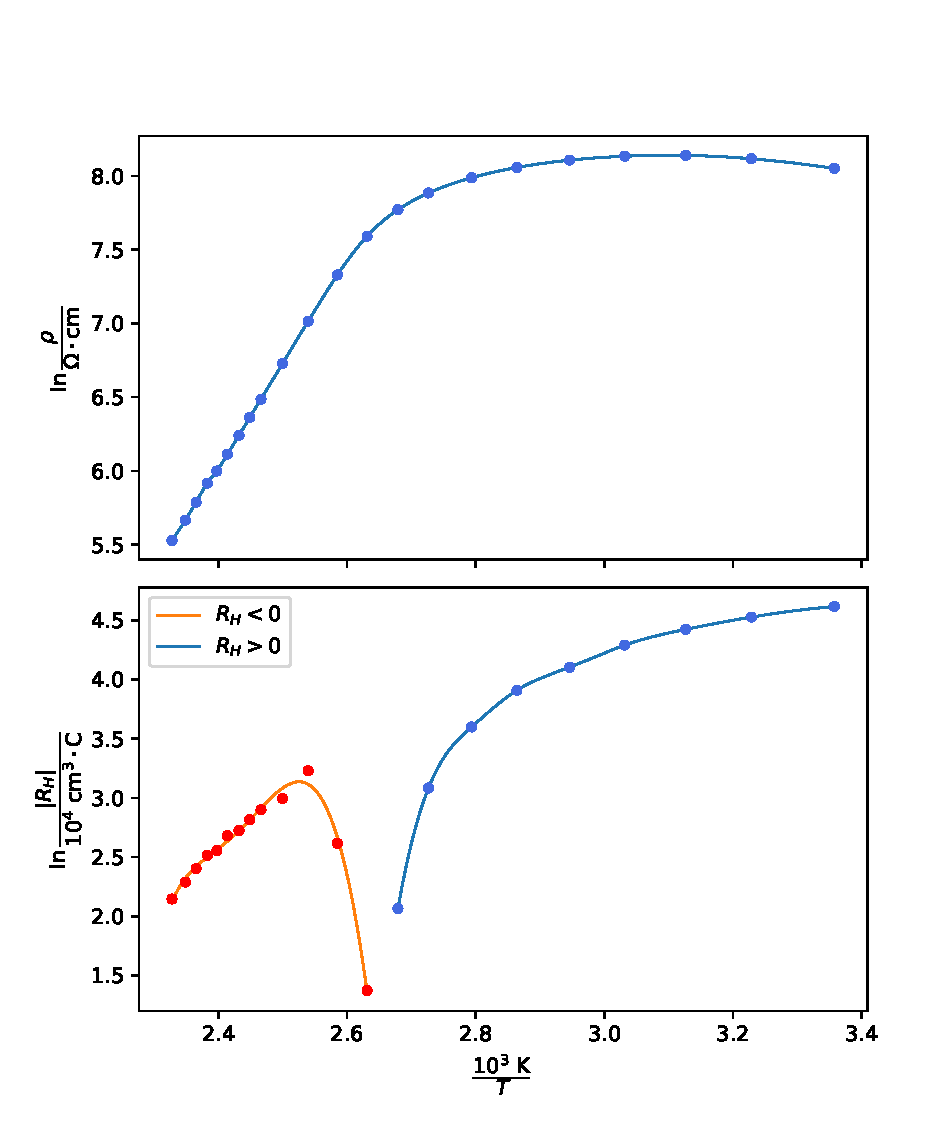
\includegraphics[width=0.8\linewidth]{fig/Tln_rho_RH.pdf}
  \caption{$\ln\rho-(1000/T)$和$\ln |R_H|-(1000/T)$曲线,根据图\ref{T_rho_RH}绘制。本图中温度$T$采用开尔文温标。因为霍尔系数$R_H=0$的时候,$\ln|R_H|\to-\infty$是奇异的,所以将$R_H<0$和$R_H>0$的区间分别进行绘制和拟合。}
  \label{Tln_rho_RH}
\end{figure}
\subsection{杂质电离饱和区}
图\ref{T_rho_RH}的测量结果中,只有前3个数据点是落在杂质电离饱和区内的。根据式\ref{mu_LP},我们可以计算这三个点对应的空穴迁移率(这里用到$(\mu_{\rm L_p})_{300}=480\ {\rm cm^2/(V\cdot s)}$,30$^\circ$C下的电阻率可由内插得到)。计算结果如表\ref{T-mu}所示。作出$\ln\mu_{\rm L_p}-\ln T$曲线并进行线性拟合,我们得到图\ref{linfit}的线性拟合图,并且我们有$$
\begin{aligned}
  \mbox{\CJKfamily{zhkai}斜率}&=-1.3,\\
  \mbox{\CJKfamily{zhkai}截距}&=13.3.
\end{aligned}
$$若假设$\mu_{\rm L_p}=AT^{-x}$,我们可以计算得到
\begin{equation}
  \begin{aligned}
    &x = -\mbox{\CJKfamily{zhkai}斜率}=1.3,\\
    &A = {\rm e}^{\mbox{\CJKfamily{zhkai}截距}}=6.0\times10^5.
  \end{aligned}
\end{equation}
\begin{table}[h]
  \centering
  \caption{根据式\ref{mu_LP}计算得到的在杂质电离饱和区内的不同温度$T$下的$\mu_{\rm L_p}$。30$^\circ$C下的电阻率是我们通过图\ref{T_rho_RH}中的数据进行内插得到的,$(\rho)_{300}=3182\ \Omega\cdot{\rm cm}$。}
  \label{T-mu}
  \setlength{\tabcolsep}{0.6cm}{
  \begin{tabular}{cc}
    \hline\hline
  $T(^\circ$C)    & $\mu_{\rm L_p}({\rm cm^2/(V\cdot s)})$    \\\hline
  24.7 & 487.2 \\
  36.6 & 456.3 \\
  46.7 & 446.0 \\\hline\hline
  \end{tabular}}
\end{table}
\begin{figure}[h]
  \centering
  \setlength{\abovecaptionskip}{-0.4cm}
  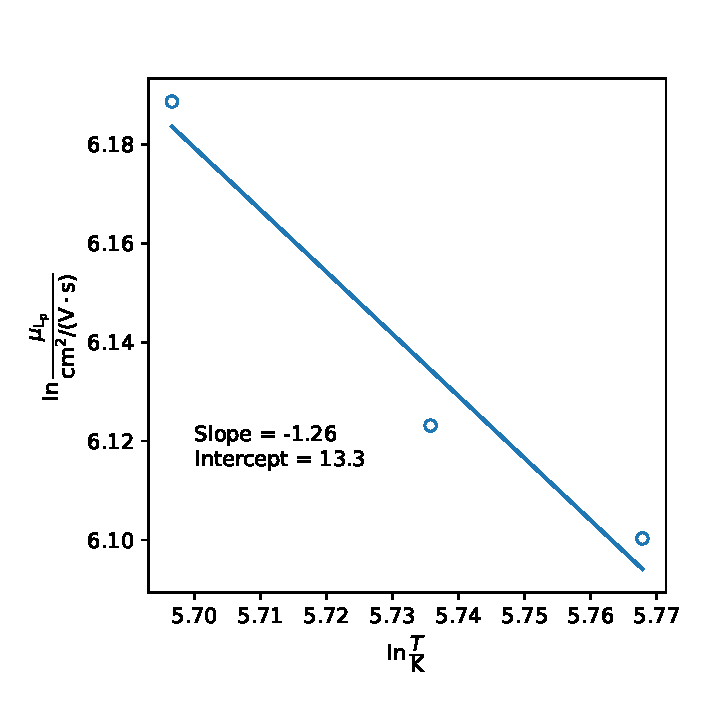
\includegraphics[width=0.5\linewidth]{fig/linfit.pdf}
  \caption{$\ln\mu_{\rm L_p}-\ln T$线性拟合图像。因为样本点比较少,所以拟合出来的结果不太尽如人意。相关系数$r=-0.98$。}
  \label{linfit}
\end{figure}

本实验给出的测定值一定和精确值有所偏离。事实上,根据前面关于霍尔系数$R_H$变化规律的分析可见,室温下实际已经有少许的本征激发(于是$R_H$随温度减小),因
此$\sigma=qN_A\mu_{\rm L_p}$在实验中的杂质电离饱和区并不严格成立。如果我们只用图\ref{T_rho_RH}的前两个点进行计算,就可以得到$$x' = -\mbox{\CJKfamily{zhkai}斜率}'=2.0,$$这显然更加接近杂质电离饱和区的情况。

为了获得更加的测量值,应该选择更低的温度进行测量,以使得在这段温度区间内霍尔系数几乎不变。但是本实验没能完成这一点,为了之后的数值计算能够准确,之后我们将直接沿用Morin等人的研究结果(式\ref{Morinresult})来计算粒子的迁移率。
\subsection{$b$值的估测}
根据式\ref{R_Hmin},我们可以通过霍尔电压的最小值$(R_H)_{\min}$估测$b$值。由图\ref{T_rho_RH}的数据可以得到$$(R_H)_{\min}=-25.3\times10^4\ {\rm cm^3\cdot C},$$将$(R_H)_{\min}$和杂质浓度$N_A$(见式\ref{NA_value})代入式\ref{R_Hmin},可以数值求解$b$,最后得到\begin{equation}
  b=2.08.
\end{equation}

而根据Morin等人的研究结果,也就是式\ref{Morinresult},我们可以直接求得$b=\mu_{\rm L_n}/\mu_{\rm L_p}$随温度变化的关系\begin{equation}\label{bex_value}
  b=\frac{\mu_{\rm L_n}}{\mu_{\rm L_p}}=16T^{-0.3}\ {\rm cm^2/(V\cdot s)}.
\end{equation}将霍尔电压取最小值$(R_H)_{\min}$时的温度$T=120.6{\rm ^\circ C}=393.7\ {\rm K}$代入上式,我们也可以直接得到\begin{equation}\label{btheo_value}
  b'=2.66.
\end{equation}

对比式\ref{bex_value}和式\ref{btheo_value},我们可以发现两者的差别是比较大的,现对其中的误差进行简单分析。

首先,我们式\ref{NA_value}中写出来的杂质$N_A$的值很有可能误差是很大的,这是因为我们计算$N_A$时使用的是杂质电离饱和区的数据,并且假定此时杂质的浓度就约等于样品中空穴的浓度,而电子的浓度近似为零。但是事实上这样的假设是有一定偏差的,室温下样品已经有一定的本征激发,这导致通过$\sigma\approx qN_A\mu_{L_p}$一式算出的$N_A$是有一定误差的。

其次,我们用到的霍尔系数的最小值$(R_H)_{\min}$可能是有偏差的。实际上霍尔系数最小值出现的温度值可能并不在我们的测量表中,所以直接用实验值得到的最小霍尔电压来代替实际上会出现的最小霍尔电压也会产生一定误差。

\subsection{禁带宽度}
这一部分我们使用Morin等人得到的结论(见式\ref{Morinresult})来估测不同温度下的空穴迁移率$\mu_{\rm L_p}$和电子迁移率$\mu_{\rm L_n}$,再根据式\ref{p_expression}就可以得到不同温度下的空穴浓度$p$和电子浓度$n$。

作$\ln p-(1000/T)$和$\ln \left(\dfrac{pn}{T^3}\right)-(1000/T)$曲线如图\ref{E_g}所示。可以发现,在本征激发的高温区,$\ln \left(\dfrac{pn}{T^3}\right)$和$(1000/T)$的线性关系比较良好,这和我们之前的理论分析一致。通过对于高温部分的线性拟合,我们就可以确定禁带宽度(见式\ref{DeltaEg})。$\ln \left(\dfrac{pn}{T^3}\right)$和$(1000/T)$的线性拟合如图所示,并且我们有$$
\begin{aligned}
  \mbox{\CJKfamily{zhkai}斜率}&=-14.0,\\
  \mbox{\CJKfamily{zhkai}截距}&=76.6.
\end{aligned}
$$由此,禁带宽度\begin{equation}
  E_g = \frac{\Delta\ln(pnT^{-3})}{\Delta \left(\dfrac{1}{kT}\right)}=-10^3k\times\mbox{\CJKfamily{zhkai}斜率}=1.21\ {\rm eV}.
\end{equation}
\begin{figure}[h]
  \centering
  \setlength{\abovecaptionskip}{-0.4cm}
  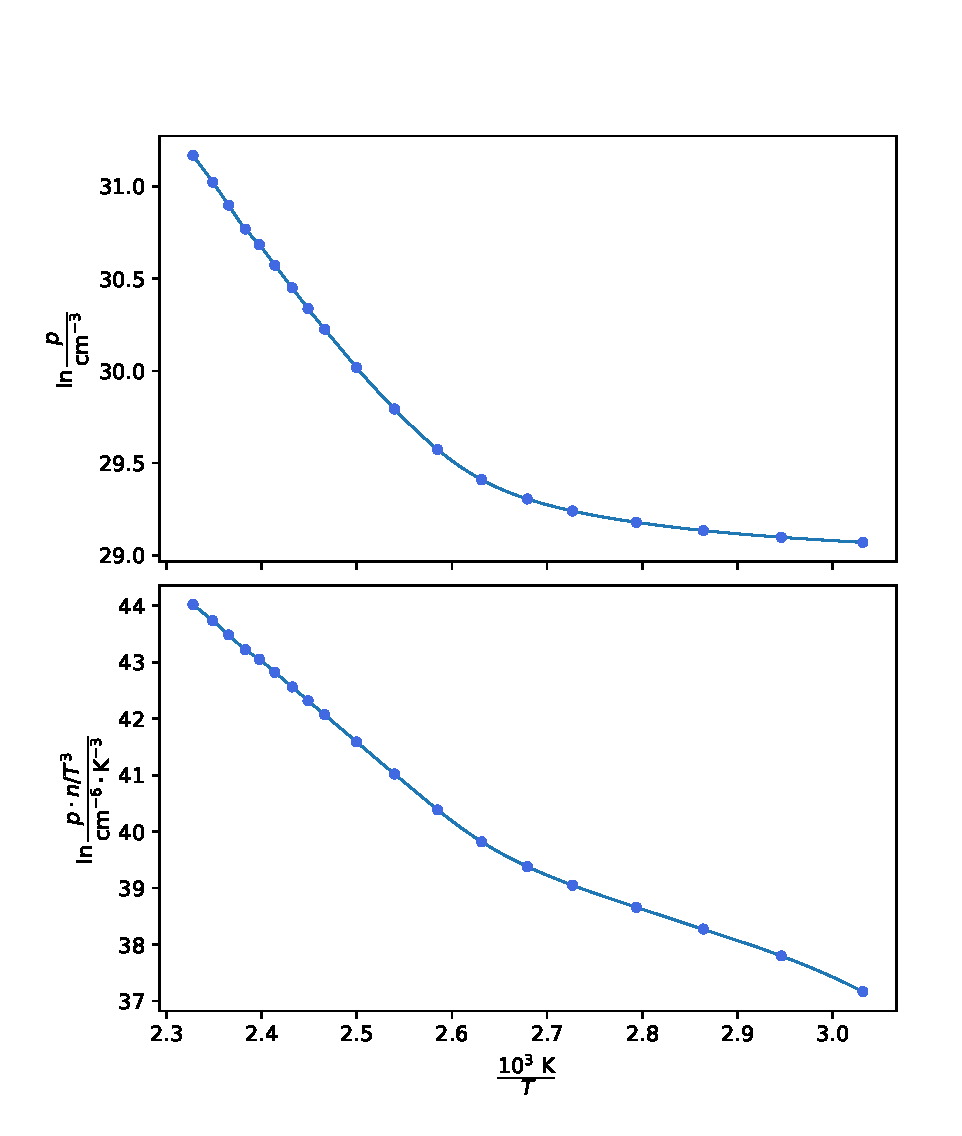
\includegraphics[width=0.8\linewidth]{fig/E_g.pdf}
  \caption{$\ln p-(1000/T)$曲线和$\ln \left(\dfrac{pn}{T^3}\right)-(1000/T)$曲线。这里只取了本征激发之后的温度范围,即从约70$^\circ$C开始。为求禁带宽度$\Delta E_g$,我们选取下图中的前半部分线性相关关系较强的部分进行线性拟合。}
  \label{E_g}
\end{figure}
\begin{figure}[h]
  \centering
  \setlength{\abovecaptionskip}{-0.4cm}
  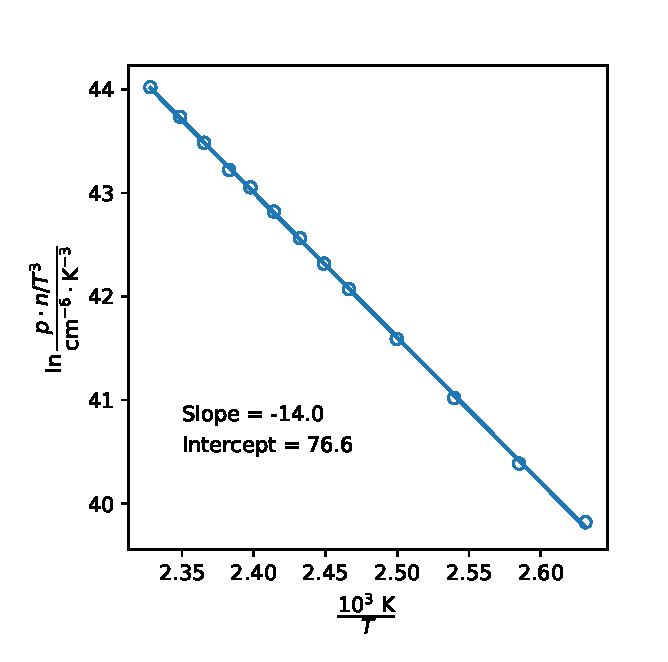
\includegraphics[width=0.5\linewidth]{fig/E_glinfit.pdf}
  \caption{$\ln \left(\dfrac{pn}{T^3}\right)$和$(1000/T)$的线性拟合图。我们只选取了前12个点进行拟合(代表本征激发比较充分的状态)。}
  \label{E_glinfit}
\end{figure}
\section{结论}
本实验通过测量从室温(\textasciitilde$25{^\circ C}$)到$160{^\circ C}$范围内p型半导体的电导率和霍尔系数。实验的温度范围为杂质电离饱和区和本征激发高温区,在这两个范围内电导率和霍尔系数的变化趋势和理论预测是一致的,由此我们初步证实了半导体理论的有效性,对半导体理论有了更进一步的理解。

在此基础上,我们进一步对实验数据进行分析,通过引用之前半导体的研究成果,我们估算了p型半导体在高温下的杂质浓度和空穴的浓度,两者相差一个数量级,由此我们知道在本实验中的高温范围内,半导体已经充分进入本征态激发;我们计算了半导体空穴的迁移率$\mu_{L_p}$随温度的变化,并和Morin等人的研究结果进行了对比,进一步给出了$b=\mu_{L_n}/\mu_{L_p}$的估测值,并进行了简单的误差分析。最后,我们计算了禁带宽度$E_g$。
\begin{acknowledgments}
  特别感谢吴孝松老师在实验过程中的指导,这使得整个实验过程更加顺利。感谢金子锟学长协力完成了本实验。
\end{acknowledgments}

\clearpage
\begin{thebibliography}{}

  \bibitem{book} 吴思诚, 荀坤. 近代物理实验(第四版). 北京: 高等教育出版社, 2015.
  \bibitem{Morin} F. J. Morin, J. P. Maita. Electrical properties of silicon containing arsenic and boron. Physical Review, 1954.96:28.
  \bibitem{Pauw} L. J. Van der Pauw, Philips Technical Review, 1958\textasciitilde1959.20,220.
  \bibitem{manual} BWH-1型霍尔效应测试仪实验手册(实验室提供)
\end{thebibliography}


\end{document}
